% USER MANUAL FOR SPOTMACHINE
%
% To compile, simply run:
% $ pdflatex usermanual.tex
% (twice to have an updated table of contents)
%
% Nice overview of most basic LaTeX commands:
% http://en.wikibooks.org/wiki/LaTeX/Document_Structure

\documentclass[a4paper,12pt]{report}
\usepackage{url,graphicx,textcomp}

\usepackage{parskip} % separate paragraphs by empty space
\setlength{\parindent}{0pt} % Do not indent first line of paragraphs

\title{SpotMachine \\ Usermanual}
\author{Thomas Pryds}
\date{June 2013}

\begin{document}

\maketitle

\tableofcontents

\chapter{Introduction}

SpotMachine lets you record and sequentially play pieces of audio. It is
intended for commercial audio spots running in shopping malls, supermarkets,
amusement parks, and other places with the need of reaching out to masses
through repetitive audio clips.

\section{Features}
There are a lot of reasons to choose SpotMachine over a dedicated piece of spot
hardware. Such devices are often very expensive, complicated to operate, and
have a limit on amount or total length of recorded spots. Following is a list of
some of SpotMachine's features.

\begin{itemize}
\item Arrange order of spots for rotation
\item Play spots by interval (specify pause time)
\item Play spots by schedule (specify point in time)
\item Record your own audio spots
\item Easy and simple user interface
\item Keep spots for later use
\item Have the same spot multiple times in the same rotation
\item No limit on number of spots or spot length
\item Audio normalization for uniform spot messages
\item Available in English and Danish (and easily extended into more languages)
%\item Upcoming: Import spot from audio file
\end{itemize}

\section{Licensing}
SpotMachine is released under the GPL license which means that you are allowed
to use it for whatever purpose you want, be it commercial or non-commercial. You
can even download the source code and change the behaviour of the program if you
so desire.

You are also allowed to redistribute SpotMachine, with or without changes, as
long as you do so under the same license, and provide the source code for
whichever changes you have made. You can read the full details of the licence in
the LICENSE text file which is distributed with SpotMachine.

\chapter{Installation}
SpotMachine runs on all major operating systems, and its only requirement is a
working, current install of Java. If you do not have Java on your system, you
should download and install it from \url{http://java.oracle.com} or through your
operating system's package management system, prior to installing SpotMachine.

You should also be able to run SpotMachine on the open source  OpenJDK instead
of the official Java from Oracle. OpenJDK is the default Java on e.g. Ubuntu Linux.

\section{Windows}
An easy-to-use installer package is available for Windows. Just download it from
the SpotMachine website, run it, and follow the instructions on-screen. The
installer, of course, provides easy, Windows-integrated means of uninstalling
SpotMachine.

\section{Ubuntu and Debian}
On systems that use the Debian packaging system, you can make use of the
precompiled deb package which is provided through the SpotMachine website. After
downloading the file, just install it by either double clicking it, or by the
following command: \texttt{sudo dpkg -i spotmachine-X.X.deb}. This package
assumes you have installed Java through the package system.

\section{Other Linux, Mac, and Others}
Currently, no installer is provided for these systems, unfortunately. However,
installation is not very complicated: Download the pre-compiled package
spotmachine*.bin.tar.bz2 (where * is the newest version number), uncompress it
to somewhere on your harddrive, and follow the instructions in the INSTALL text
file.

\section{Sources}
If you wish to compile SpotMachine yourself, you can download the source code
package from the SpotMachine website. Uncompress the file to somewhere on your
harddrive, and follow the instructions in the INSTALL text file.

\chapter{Daily Usage}
All features of SpotMachine are, directly or indirectly, available from the main
window. This is where you can see an overview of recorded spots, which spots are
currently in rotation, when they are playing.

\begin{figure}[h]
\centering 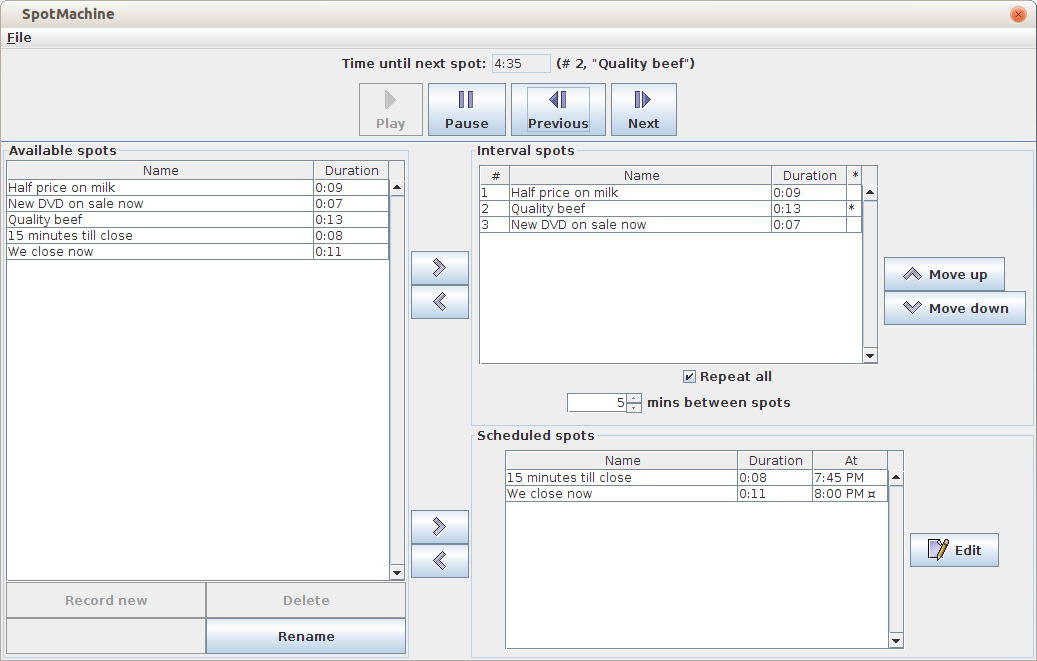
\includegraphics[width=130mm]{mainwindow.png}
\caption{Main window}
\end{figure}

The main window is split up in three parts:
\begin{itemize}
\item The top part containing the {\bf control buttons} Play, Pause, Previous
      and Next.
\item The left side containing all {\bf available spots}.
\item The right side containing spots currently in {\bf interval rotation} and
      spots currently in {\bf scheduled rotation}.
\end{itemize}

\section{Control Buttons}
At the top you control whether the current rotation spots are to be played, or
if they're on pause. For normal use, the SpotMachine would typically be set to
``Play'' and then left alone. Pause would typically be used while recording new
spots -- in fact you cannot record new spots, unless pause in on. Note that
pausing only affects spots that are on interval rotation (see further down for
an explanation), not those set for scheduled play. %This behaviour might change

\section{Available Spots}
The left side of the main window shows a list of recorded spots. These spots are
not necessarily set up for interval or scheduled play (more about this later) --
this is a list of all spots available to you at any given moment. By selecting a
spot in this list, you may rename it, delete it, or set it up for interval or
scheduled play.

\subsection{Recording a New Spot}
You can record a new spot through a connected microphone. All new spots will
show up in the Available spots list. To do so, click the Record new button below
the Available spots list, and a new window will pop up, from which you can
control the recording itself.

\begin{figure}[h]
\centering 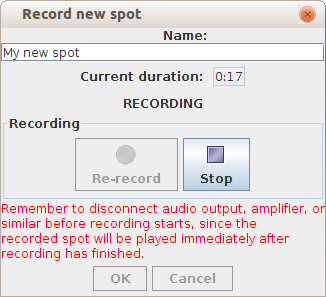
\includegraphics[width=50mm]{recorddialogue.png}
\caption{Record new spot window}
\end{figure}

Here, you can give the spot a name, which will appear in spot lists. Be sure to
give the spot a descriptive name, and note that you {\em are} able to give the
exact same name to two different spots! You are able to type in a name either
before, during or after recording a spot.

In the middle of the window are two buttons. The left button will start the
actual recording of the spot. The right one will stop recording. While
recording, you can keep track of the length of the spot just above the record
and stop buttons. Here, you can also see, whether SpotMachine is currently
recording, or not.

When you click the Stop button, the recording is immediately played back once,
to let you hear if everything is like you want it to be. For this reason, be
sure to check that you are not connected to an amplifier or in some other way
publicly transmitting before starting to record new spots. Connecting a set of
headphones instead is recommended. If the recording does not sound ok, you can
click the record button again, which discards the previous recording and starts
a new one.

If you like what you hear, click the OK button, and the new spot is added to the
Available spots list in the main window. If instead, you click the Cancel
button, any newly recorded spot is discarded, and the recording window is
closed.

\subsection{Deleting a Spot}

\begin{figure}[h]
\centering 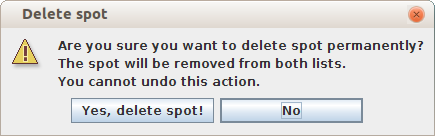
\includegraphics[width=60mm]{deletespotdialogue.png}
\caption{Delete spot window}
\end{figure}

If you decide you will not need a certain spot ever again, you can delete it
entirely from disk. You do so by selecting the spot in the Available spots list
and click the Delete button. You will be met with a brief acknowledge window,
just to make sure that you are not deleting something by accident. If you delete
a spot that is currently also in the Interval spots and/or Scheduled spots
lists, the spot will also be removed from these lists.

Note, this function deletes the spot's audio file from disk, so it is
non-reversible. If you are probably going to use a spot at some later point, but
not now, you can just let it sit in the Available spots list for later use.

\subsection{Renaming a Spot}

\begin{figure}[h]
\centering 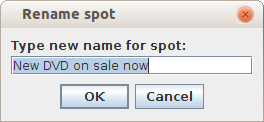
\includegraphics[width=40mm]{renamespotdialogue.png}
\caption{Rename spot window}
\end{figure}

Changing the name of a spot after it has been recorded is possible through the
Rename button. By clicking it you will be presented with a small popup window
that allows you to do so. Bear in mind, that spots are not recognized by the
program from their names, so it is perfectly possible to name two spots exactly
the same, for whatever reason you might have to do so. In most cases, this is
discouraged, though, as to not confuse spots with each other.

\section{Interval and Scheduled Spots}
The right side of the main window is, in turn, divided into two lists of spots.
The spots shown in these two lists have the fact in common that they are set up
for being played in one way or another; playlists, if you like. Note, that a
spot can easily appear in both lists -- in fact, it can appear more than once in
either list.

\paragraph{Interval spots:} The first one is a list of spots that are played
sequentially with a given interval between them, e.g. five minutes. In a
commercial setting like a supermarket, this would be used for promoting special
offers (``Half price on milk today''), service announcements (``Extended opening
hours tomorrow''), etc. In figure~\ref{intervalspotslist} you see an example of
a list of interval spots. They are presented in the order they will be played,
and the asterisk (*) on one of the lines tells you which spot will be played
next.

\begin{figure}[h]
\centering 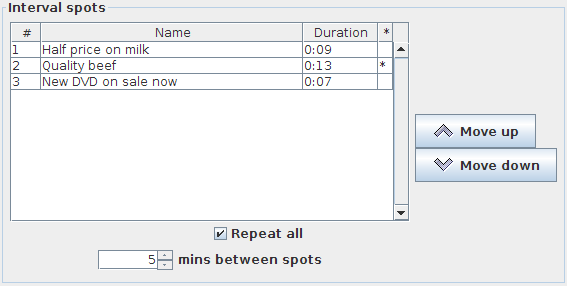
\includegraphics[width=70mm]{intervalspotslist.png}
\caption{Interval spots list}
\label{intervalspotslist}
\end{figure}

\paragraph{Scheduled spots:} The second list contains spots which are played at
a given point in time, e.g. at 7:45~PM every Monday to Friday. This might be
used for time based service announcements (like in our supermarket example: ``15
minutes till closing time'', etc.). Figure~\ref{scheduledspotslist} shows an
example of a scheduled spots list. Some lines may show a ``\textcurrency''
symbol. This means that the spot has been configured to run only on certain,
defined days. This will be explained in more detail in
section~\ref{sec:addscheduledspot}.

\begin{figure}[h]
\centering 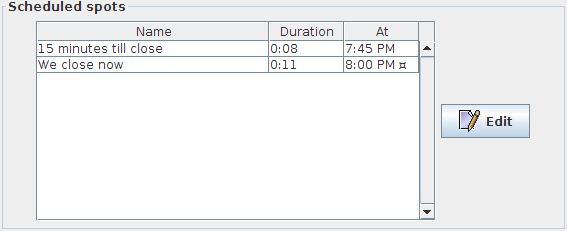
\includegraphics[width=70mm]{scheduledspotslist.png}
\caption{Scheduled spots list}
\label{scheduledspotslist}
\end{figure}

\subsection{Adding a Spot as an Interval Spot}
Between the Available spots list and the Interval spots list, you see two arrow
buttons. The arrow point to the right copies a spot into the Interval spots
list. You can copy the same spot into the list several times, if you have a
certain spot that you want to play more often than the others.

\subsection{Changing the Properties of Interval Spots}
The play order is given in the list, and by selecting a spot and clicking the
Move up and Move down buttons, you can change this to your linking.

Below the list you can choose whether to start over when the end of the list has
been reached (by checking the Repeat all checkbox). Also, you can set the amount
of minutes between playing each spot.

\subsection{Adding a Spot as a Scheduled Spot}
\label{sec:addscheduledspot}
Like for interval spots, there are two arrow buttons for scheduled spots. The
right-pointing arrow copies a spot to the Scheduled spots list, while the
left-pointing arrow removes it.

\begin{figure}[h]
\centering 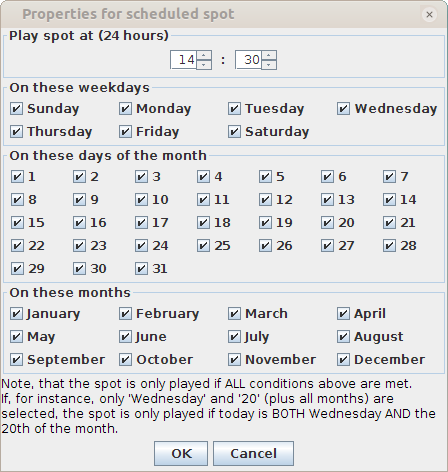
\includegraphics[width=70mm]{scheduledspotdialogue.png}
\caption{Adding a scheduled spot}
\end{figure}

When you add a spot to the Scheduled spots list, you are presented with a
properties window which mighy look confusing at first. Actually, it is quite
simple, though. The first part sets the time of day (always in 24 hour system)
for the spot to start playing. Then come weekdays, day of the month, and month.

For a group (for instance ``weekdays'') either of your selections may be true in
order for the spot to play. In figure~\ref{scheduledspotexample1}, the spot will
play if today is either Monday or Tuesday. It should be quite clear that this
works as ``OR'', and not as ``AND'', since it will never be both Monday and
Tuesday on the same day.

\begin{figure}[h]
\centering 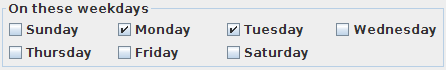
\includegraphics[width=70mm]{scheduledspotexample1.png}
\caption{Weekdays example}
\label{scheduledspotexample1}
\end{figure}

What is important to notice is that between groups, the relation is ``AND''.
This means that in figure~\ref{scheduledspotexample2}, the spot will play if
today is either Monday or Tuesday, AND at the same time it is the 15th of the
month. Or put the other way around: The spot will play on the 15th, but only if
the 15th is a Monday or a Tuesday. This means that if you want the spot to play
on all Mondays and Tuesdays, but also on all of the 15th, you will have to add
the spot twice.

\begin{figure}[h]
\centering 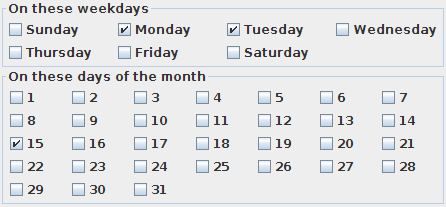
\includegraphics[width=70mm]{scheduledspotexample2.png}
\caption{Weekdays and day of the month example}
\label{scheduledspotexample2}
\end{figure}

\subsection{Changing the Properties of Scheduled Spots}
Once a scheduled spot has been added, it is possible to bring back the
properties window. This is done by selecting the spot that you want to change,
and then clicking the Edit button next to the spot list. Here you will be able
to edit all the details as described in the above section.

\section{Preferences}


\section{Less Obvious Options}

\subsection{Editing of Spot Sound Files by Third-Party Programs}

If you wish to do so, it is possible to edit the sound files that were recorded
in SpotMachine, or even replace a spot altogether, through third-party software,
such as Audacity. The edited/replacing spot doesn't have to be the same length
or even format as the original. It does have to be an uncompressed WAV-file,
though. You might wish to do this if you want to apply some more sofisticated
effects or filters to a the sound file than what SpotMachine can deliver.

This is a feature that is not yet implemented as such, so it is basically a
question of closing down SpotMachine (important, as to not confuse it about
changing spot lengths, audio formats, etc.), then locating the actual sound
files on disk and opening them in your third-party sound editor of choice.

On Linux and Mac, the sound files will be present in a directory
\texttt{.spotmachine} in the user's home directory. On Windows, the directory
will most likely be present in the system's default location for application
data. This is a bit different on different versions and translations of Windows,
so the easiest way to locate the directory on your system is probably to open
the file explorer, type \texttt{\%programdata\%}, and hit enter.

The files will have random names, but perhaps you can recognize the one you
want on the file's creation date/time. Remember to save the file with the exact
same file name (including the \texttt{.wav} extension).

SpotMachine records spots in uncompressed PCM format (signed), with a sample
rate of 44,100 Hz, in 16 bits mono, but is capable of playing PCM files with
other sample rates, bits, mono/stereo, etc. It will not be able to play
compressed files, such as MP3 files, though.

\subsection{Forcing a Certain Sound Mixer}
% From NEWS file:
%- Output and recording mixers can be forced through the Java prefs file for SpotMachine.
%  If a key called ForcePlayOnMixerNumber contains a value > 0 representing a valid mixer number,
%  that mixer will be used (if applicaple)for playing spots instead of the default one.
%  The same goes for recording spots, except here the key is called ForceRecordingOnMixerNumber.

\chapter{Contributing}

SpotMachine is open source software. That means, among other things, that at all
times you have access to the source code from SpotMachine's website. Having
access to that, you may choose to contribute.

There are several ways you can contribute. Also ways that don't require you to
be a programmer, or even technically minded.

% Reporting bugs if you find any
% Translating
% Code

\end{document}

